%!TEX root = ../thesis.tex
%5-NIR-information

\chapter{NIR information}  % Main chapter title

\label{cha:nir_content}

%----------------------------------------------------------------------------------------
%	SECTION 1
%----------------------------------------------------------------------------------------

\section{Radial velocity precision}
The first detections of planets with the RV technique \textbf{Queloz 2995} discovered the mass and close in hot-Jupiter planets. These are the easiest to detect with the highest RV amplitude.

Over the years the community has push the limits of this technique to smaller and smaller planetary masses. An example is shown in Fig.~\ref{fig:year_mass}. 
\begin{figure}
\label{fig:year_mass}
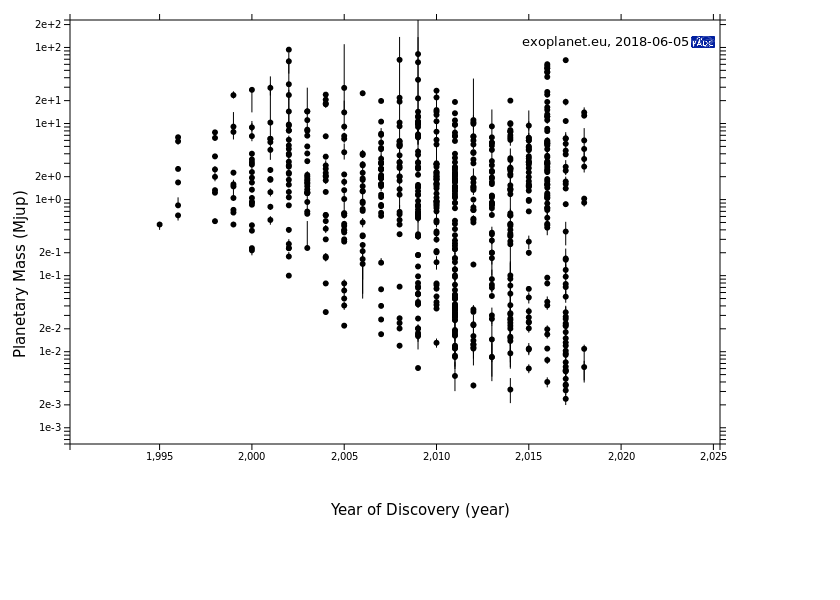
\includegraphics[width=0.8\linewidth]{figures/year_planet_mass.png}
\caption{Mass of discovered planets verse year. From Exoplanet.eu}
\end{figure}


RV amplitude scales with mass of the star $M_\star^{-2/3}$ and with the planetary orbital period $P_\textrm{orb}^{-2/3}$.

The detection of an Earth-mass planet inside the habitable zone around a solar-type star, the RV amplitude is 10 cm/s. If that a planet with the same characteristics is instead orbiting a M/ -dwarf, the RV amplitude is larger than 1 m/s. This is due to two factors, the smaller mass of the host star, and the closer habitable zone, due to a lower luminosity output of the host)

\citet{artigau_optical_2018} recently compared archival spectra of Barnard's Star, an M-dwarf, and found that state-of-the-art atmosphere models over-predict the $Y$ and $J$-band RV content by more than a factor of $\sim$$2$, while under-predicting the $H$ and $K$-band content by half.

We are currently aiming to extend this work over the whole M-dwarf range, from M0-M9.


History of Precision calculations:
Connes 1985 -
Bouchy et al. 2001  - photon noise limit on rv measurements.   
Figueria et al. 2016 - focus on m-dwarfs parameter range to specify new instrumentation windows to focus.
Reiners 2017 -  Carmenes sample. some precision



%-----------------------------------
%	SUBSECTION 1
%-----------------------------------
\subsection{Fundamental photon noise limitation}
A optimum technique to calculate the radial velocity precision of s spectrum using the full spectral information is proposed by \citet{Connes1985}. For each spectrum there is assigned a quality factor, Q, to compute the fundamental uncertainty on the radial velocity measurements due to noise.

\begin{figure}
    \centering
    %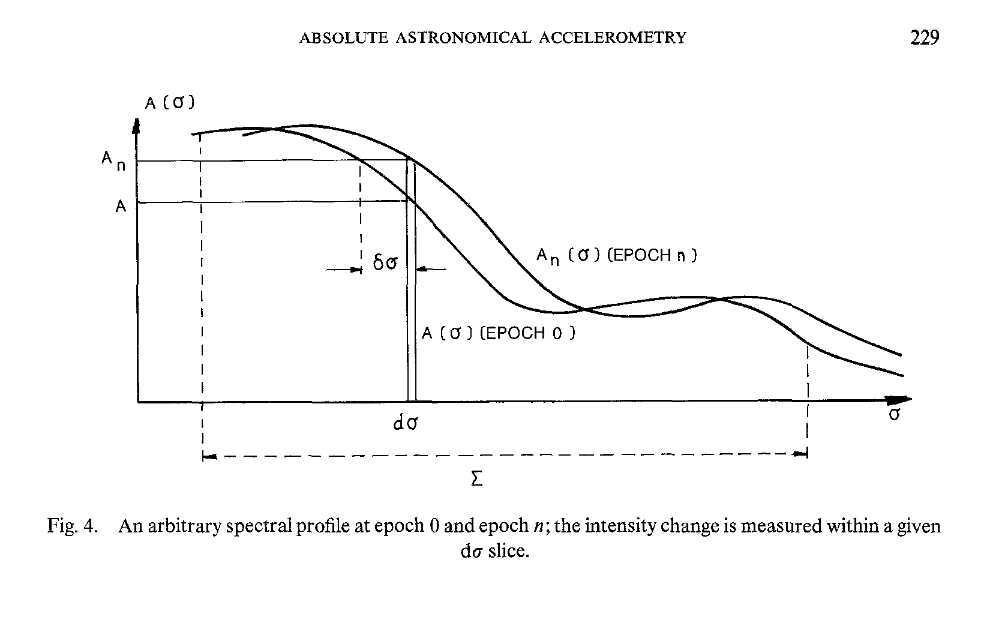
\includegraphics[width=0.7\linewidth]{figures/spectrum_example_a}
    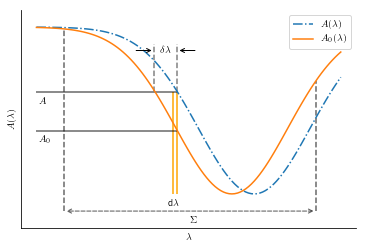
\includegraphics[width=0.7\linewidth]{figures/precision_derivation}
    \caption{Arbitrary spectral line with a shift $\delta \lambda$, inspired by \citet{Connes1985}.}
    \label{fig:precisionderivation}
\end{figure}

Here we explain the derivation following \citet{Connes1985, bouchy_fundamental_2001, figueira_radial_2016}. A mix of notations from each is used with some extra notes to try and make things clear.

The Doppler shift of a spectrum is given by:
\begin{equation}
\frac{\delta V}{c} = \frac{\delta \lambda}{\lambda}.
\label{eq:dopplershift}
\end{equation}
Here $c$ is the speed of light in a vacuum, and $\delta \lambda$ is the observed shift in wavelength $\lambda$ caused by the velocity $\delta V$

Using basic calculus \(\delta y = \frac{\partial y}{\partial x} \delta x,  \nonumber\) and for a Doppler shift that is small compared to the line-width\footnote{Although \textbf{Connes 1983} show that this approximation in Eq.\,\ref{eq:intensitychange} is adequate under all circumstances}, the observable intensity change at a given pixel can be expressed by:

\begin{equation}
\delta A(i) = A(i) - A_0(i) \simeq \frac{\partial A_0(i)}{\partial \lambda} \delta \lambda
\label{eq:intensitychange}
\end{equation}

Rearranging Eq.~\ref{eq:intensitychange} for \(\delta \lambda\) and putting it into Eq.~\ref{eq:dopplershift}, the Doppler shift of then becomes:
\begin{equation}
    \frac{\delta V(i)}{c} = \frac{A(i) - A_0(i) }{\lambda(i) (\partial A_0(i)/\partial \lambda(i))}
\end{equation}

This equation shows that the changes in velocity is measured through a change in intensity in the recorded spectrum, \(A(i)-A_0(i)\), and inversely proportional to the slope of the spectrum, \(\partial A_0(i)/\partial \lambda(i))\). 
This equation provides a measurement of the radial velocity shift for each pixel (i) in the spectrum. The whole available spectral range, $\Sigma$, should be used to increase the sensitivity of the measurement and decrease the noise. This is achieved with a weighted average, by summing the contribution of all pixels using an optimal weight W(i).

\begin{equation}
\frac{\delta V}{c} = \frac{\Sigma{ \frac{\delta V(i)}{c}W(i)}}{\Sigma {W(i)}}
\end{equation}

\citet{Connes1985} show that the optimal weights for photon limited noise is given by.....

There is also a optimal weight for detector noise but we are always assume we are in high SNR case and are photon noise limited.

 zero rv measurement to get precision? Connes relevant here...?

Statistically, the optimal weights are proportional to the inverse square of the individual dispersion,

\begin{equation}
W(i) = \frac{1}{\left(\frac{\delta V_{RMS}(i)}{c}\right)^2},
\end{equation}
where $X_{RMS}$ is the dispersion on the quantity $X$.


given photon noise.... is given by Connes 1985... 


\begin{equation}
    \frac{\delta V_{RMS}}{c} = \frac{1}{\Sigma {W(i)}} = \frac{1}{Q \Sigma {A_0(i)}}
\end{equation}

\begin{equation}
Q = \frac{\sqrt{(\Sigma{W(i)}}}{\sqrt{\Sigma{A_0(i)}}}
\end{equation}

Considering that \(\Sigma{A_0(i)} = N_{e^-} \) is the total number of photoelectrons counted over the whole spectral range then the uncertainty in the velocity change is finally given by:

\begin{equation}
\frac{\delta V_{RMS}}{c} = \frac{c}{Q \sqrt{N_{e^-}}} = \frac{c}{Q S/N}.
\end{equation}

In the photon noise dominated region the \(\sqrt{N_{e^-}} = S/N\), signal-to-noise of the detection. \unfinished{It is convenient to use this version when comparing observed spectra with different S/N.?} 


\begin{equation}
\bar{\delta V_{RMS}} = \frac{1}{\sqrt{\Sigma{(\frac{1}{\delta V_{RMS}(k)})^2}}}
\end{equation}



\subsection{Prepare phoenix aces models}:
\# see Figuria 2016

Convert SED to counts.


Scale to 100 snr per resolution element in J band.

Convolutions


Since the synthetic models do not have a consistent wavelength grid, the discretization of the convolution kernel onto the  changing wavelength grid causes each pixel to be multiplied by  a slightly different kernel area. We therefore divide the result by a convolution of a spectrum of ones with the same wavelength resolution.


%-----------------------------------
%	SUBSECTION 2
%-----------------------------------

\subsection{Comparing models to Carmenes.}
Already somewhat done in Reiners. (use all spectra).

Band by band like Figueria 2016?
Certain\% steps like Bouchy or Artigau


Can do Barnards star in Carmenes. compared to models in Artigau.



%----------------------------------------------------------------------------------------
%	SECTION 2
%----------------------------------------------------------------------------------------

\section{Main Section 2}



\section{Code improvements}
Care needs to be taken to optimize the code. The original code used in Figueira 2016 was very slow, taking around 2 hours per simulation, this lead to weeks of processing time to compute the precision's for the paper.

Some work focused on testing ideology from computer science. Although not perfect implementation I began by adding automated tests to the code to check individual parts of it. 
Before making changes I created automated tests that would confirm the functionality of pieces of the code. I could then make changes to the code, to improve the performance without worrying that the results were different.
Namely that the same precision were calculated in the end.

There was a major performance bottleneck in the convolution stage, which increased the performance around 250X itself. The algorithm looped though the pixels in the spectrum, selecting out the necessary section around a given pixel with a comprehension list (for loop if inside range). Turning the result into a numpy array, performing the sum for that pixel and appending it to a list. 

\textbf{Insert code samples.}

\begin{lstlisting}[language=Python, caption=Python example old]

def pixel_rot_convolution(wl_0, wl, flux, vsini, epsilon):
flux_conv_rot = []
counter=0
    for wl_0 in wav_extended:
        # select all values such that are within the FWHM limits
        delta_wl = wl_0*vsini/3.0e5
        mask = [i for i in range(len(wal)) if
                         ((wl_0 - delta_wl) < wl[i] < (wl_0 + delta_wl))]
        flux_2convolve = flux[mask[0]:mask[-1]+1]
        rotation_profile = rotation_kernel(wl[mask[0]:mask[-1]+1] - wl_0, delta_wl, vsini, epsilon)
        flux_conv_rot.append(np.sum(rotation_profile*flux_2convolve))
 
flux_conv_rot = np.array(flux_conv_rot, dtype="float64")

\end{lstlisting}

These simple examples ignore the edge effects which are incorporated, by extending the wavelength range used by 5 fwhm.
\begin{lstlisting}[language=Python, caption=Python example]

flux_conv_rot = np.empty_like(wl)
for i, wl_0 in enumerate(wl):
    """Rotational convolution for pixel wl_0."""
    # select all values such that they are within the fwhm limits
    delta_wl = wl_0 * vsini / 3.0e5

    mask = (wl > (wl_0 - delta_wl) &  (wl < (wl + delta_wl)))
    rotation_profile = rotation_kernel(wl[index_mask] - wl_0, delta_wl, vsini, epsilon)
    
    pixel_conv = np.sum(rotation_profile *  flux[mask]) / np.sum(rotation_profile)
    flux_conv_rot[i] = pixel_conv

\end{lstlisting}


\begin{lstlisting}

def rotation_kernel(delta_lambdas: ndarray, delta_lambda_l: float, vsini: float, epsilon: float) -> ndarray:
"""Calculate the rotation kernel for a given wavelength

Parameters
----------
delta_lambdas: array
Wavelength values selected within delta_lambda_l around central value. (check)
delta_lambda_l: float
FWHM of rotational broadening. (check)
vsini: float
Projected rotational velocity [km/s]
epsilon: float
Linear limb-darkening coefficient (0-1).

Returns
-------
Rotational kernel

Notes:
Equations * from .... book.

"""
denominator = (np.pi * vsini * (1.0 - epsilon / 3.0))
lambda_ratio_sqr = (delta_lambdas / delta_lambda_l) ** 2.0

c1 = 2.0 * (1.0 - epsilon) / denominator
c2 = 0.5 * np.pi * epsilon / denominator

return c1 * np.sqrt(1.0 - lambda_ratio_sqr) + c2 * (1.0 - lambda_ratio_sqr)
\end{lstlisting}

The solution is to iterate over each pixel but create a mask array and use numpy indexing to select the required pixel span. (this remains in numpy ) 
These operations all remain in numpy so do not waste time converting between lists and numpy arrays, in which Python need to constantly check and convert the type of each item.

This shows a lesson in the usefulness of test driven development, or testing of code in science.


An normalization step was originally done after the convolution, to normalize out the effect of the convolution on a spectrum of 1s, due to the changing wavelength grids sampling. This was brought inside the main convolution by dividing the pixel by the convolution of a spectrum of ones at the same time. (again in numpy so it is quick)

Parallelization as embarrassingly parallel, the result of each pixel is independent of result of neighbors.

This is not a criticism of the work done by the original author (my supervisor). It is easier to modify a working system then to create one from scratch.

Computer code is not the important part in scientific exploration., although becoming more important in open source and reproducibility efforts. Often forgotten in 

\# Handle any phoenix aces models.


\section{SPIRou and NIRPS ETC}
Having this tool to calculate RV precisions efficiently lead to contributions to the Exposure Time Calculators (ETC) for both the SPIRou and NIRPS spectrographs.

In Septemeber 2017 we were requested to provide precision calculations for the SPIRou ETC\footnote{\url{http://www.cfht.hawaii.edu/Instruments/SPIRou/SPIRou_etc.php}}. These were the same table as \citet{figueira_radial_2016} but with a each band referenced to 100 SNR in its own band. The modification to use the center of any band was made to fulfill this request. Notes on the telluric correction issue affect on Condition. 2.  

In May 2018 we were requested to provide precision calculations for the NIRPS ETC. This extended the spectral range from M0, M3, M6, M9 at 3900. 3500, 2800 2600 K respectively, but to all temperatures between 2500 and 4000K inclusively. This provides a finer resolution coverage over the M spectral type, allowed by the PHOENIX-ACES library.
Instrumental resolutions of 75000 and 100000 were requested to match the NIRPS instrument.
The logg and metallicity, sampling rate remained at the \citet{figueira_radial_2016} levels of 4.5, 0.0 and 3 respectively.
Precisions were provided for SNR of 100 relative to the J, H bands as well as to each band individually. Artigua 2018.(priv. communication) suggested the truly relevant value is the SNR in H band for NIRPS radial velocities.

A table of the precisions created for the NIRPS ETC are provided as an online table to our publication \textit{Neal et al. 2018b (in prep.)} \footnote{Available at \url{}.} \unfinished{Inlcude correct links} 

